\chapter{Teoría de ciclos límite}

En el estudio cualitativo de sistemas dinámicos no lineales, los \textit{ciclos límite} juegan un papel fundamental al describir comportamientos periódicos estables o inestables que no dependen de las condiciones iniciales específicas del sistema. Estos ciclos representan soluciones cerradas aisladas en el plano fase, lo que los convierte en objetos clave para entender fenómenos oscilatorios en diversas áreas de aplicación.\\

El análisis de la existencia y estabilidad de ciclos límite está íntimamente ligado al famoso \textit{Teorema de Poincaré-Bendixson}, uno de los resultados más importantes en la teoría de sistemas dinámicos planos. Este teorema proporciona las condiciones bajo las cuales las trayectorias de un sistema bidimensional acotado convergen hacia un conjunto límite, ya sea un punto de equilibrio o una órbita periódica. Su relevancia radica en que permite descartar comportamientos caóticos en sistemas planos y ofrece herramientas rigurosas para identificar ciclos límite.\\

En este capítulo, nos enfocamos en el desarrollo teórico de los ciclos límite y presentamos el Teorema de Poincaré-Bendixson como una herramienta central para su estudio.

\section{Sistemas dinámicos}

Dado un sistema autónomo de ecuaciones diferenciales ordinarias
\begin{equation}\label{eq: sistAuto}
	\begin{matrix}
		x(t)'= F(x(t))\\
		x(0)=x_0
	\end{matrix}
\end{equation}
con $F\in C^1(D)$ y $D\subset\mathbb{R}^n$ un conjunto abierto, sabemos que este tiene una única solución $\varphi^t(x_0)=x(t)$ para cada condición inicial $x_0\in D$, para todo $t\in I(x_0)$, máximo intervalo de existencia de la solución. La solución $\varphi^t(x_0)$ se llama flujo del sistema y satisface que $\varphi^0(x_0)=x_0$ y $\varphi^t(\varphi^s(x_0))=\varphi^{t+s}(x_0)$ para todo $x_0\in D$ y $t,s\in I(x_0)$. \cite{perko2001differential}. \\

Vamos a definir los sistemas dinámicos, así mismo vamos a abordar un teorema que nos permite extender en máximo intervalo de existencia de la solución.
 
\begin{definition}[Sistema dinámico]
	Sea $D\subset\mathbb{R}^n$ un conjunto abierto, un sistema dinámico en $D$ es una familia de aplicaciones continuas $C^1$
	$$\varphi:D\times\mathbb{R}^n\to\mathbb{R}^n$$
	tal que si $\varphi^t(x)=\varphi(t,x)$, entonces $\varphi^t$ satisface:
	\begin{enumerate}
		\item $\varphi^0(x)=x$ para todo $x\in D$
		\item $\varphi^t(\varphi^s(x))=\varphi^{t+s}(x)$ para todo $x\in D$ y $t,s\in\mathbb{R}$
	\end{enumerate}
\end{definition}

Si $\varphi(t,x)$ es un sistema dinámico en $D\subset\mathbb{R}^n$ y sea 
$$F(x)= \frac{\partial\varphi}{\partial t}(t,x)|_{t=0}$$
entonces $f$ es un campo vectorial en $D$ y se llama campo vectorial asociado al sistema dinámico $\varphi(t,x)$. Además $\varphi(t,x_0)$ es solución del problema de valor inicial
\begin{equation}\label{eq: sisAuto}
	\begin{matrix}
		x(t)'= F(x(t))\\
		x(0)=x_0
	\end{matrix}
\end{equation}

\begin{definition}[Sistemas topológicamente equivalentes]
	Sean dos sistemas de ecuaciones diferenciales ordinarias
	\begin{equation}\label{eq: sis1}
		x'=f(x)
	\end{equation}
	\begin{equation}\label{eq: sis2}
		x'=g(x)
	\end{equation}
	con $f\in C^1(D)$ y $g\in C^1(E)$, $D,E\subset\mathbb{R}^n$ conjuntos abiertos. Decimos que los sistemas $\eqref{eq: sis1}$ y $\eqref{eq: sis2}$ son topológicamente equivalentes si existe un homeomorfismo $h:D\to E$ tal que mapea trayectorias de $\eqref{eq: sis1}$ en trayectorias de $\eqref{eq: sis2}$ y viceversa, además preserva el sentido de las trayectorias.
\end{definition}

\begin{definition}[Teorema de existencia global]
	El problema de valor inicial
	\begin{equation}\label{eq: sisAuto}
		\begin{matrix}
			x(t)'= \frac{F(x(t))}{1+|F(x(t))|}\\
			x(0)=x_0
		\end{matrix}
	\end{equation}
	tiene solución única para todo $x_0\in D$ y $t\in I(x_0)=(-\infty,\infty)$ máximo intervalo de existencia de la solución. \cite{perko2001differential} Además es topológicamente equivalente al sistema \eqref{eq: sisAuto} en $\mathbb{R}^n$.
\end{definition}

\begin{definition}[Conjunto invariante]
	Un conjunto $U\subset\mathbb{R}^n$ es invariante bajo el flujo $\varphi^t$ si para todo $x\in U$ se tiene que $\varphi^t(x)\in U$ para todo $t\in\mathbb{R}$.
\end{definition}

\section{Conjuntos límite}

Consideremos el sistema de ecuaciones diferenciales ordinarias

\begin{equation}\label{eq: sis1}
	\begin{matrix}
		x'=-y+x(1-x^2-y^2) \\
		y'=x+y(1-x^2-y^2)
	\end{matrix}
\end{equation}

con las condiciones iniciales $x(0)=x_0$, $y(0)=y_0$.\\

Para realizar un análisis cualitativo del sistema vamos a hacer un cambio
de coordenadas de cartesianas a polares, con el fin de simplificar
el sistema \cite{perko2001differential}, después vamos a resolver cuantitativamente el problema y
analizaremos algunas propiedades con ayuda de la solución analítica.\\

Con el cambio de coordenadas $\eqref{eq: xpolar}$ y  $\eqref{eq: ypolar}$ tenemos
las condiciones iniciales $r(0)=r_0=\sqrt{x_0^2+y_0^2}$ y $\theta(0)=\theta_0=\arctan(\frac{y_0}{x_0})$.\\

Sustituimos el sistema $\eqref{eq: sis1}$ en $\eqref{eq: drcart}$:
$$rr'=xx'+yy'=x[-y+x(1-x^2-y^2)]+y[x+y(1-x^2-y^2)]$$
$$rr'=x^2(1-x^2-y^2)+y^2(1-x^2-y^2)=(x^2+y^2)[1-(x^2+y^2)]$$
luego sustitituimos $\eqref{eq: r2}$ y obtenemos la ecuación diferencial
$$rr'=r^2(1-r^2)$$
\begin{equation}\label{eq: drsis1}
	r'=r(1-r^2)
\end{equation}\\

Por otro lado sustituimos el sistema $\eqref{eq: sis1}$ en $\eqref{eq: dthetacart}$:
$$r^2\theta'=xx'-yy'=x[x+y(1-x^2-y^2)]-y[-y+x(1-x^2-y^2)]$$
$$r^2\theta'=x^2+y^2=r^2$$
y obtenemos la ecuación diferencial
\begin{equation}\label{eq: dthetasis1}
	\theta'=1
\end{equation}

Las ecuaciones $\eqref{eq: drsis1}$ y $\eqref{eq: dthetasis1}$
forman un sistema de ecuaciones no lineal desacoplado \cite{strogatz2018nonlinear}.\\

Comenzamos el análisis cualitativo de la ecuación diferencial $\eqref{eq: drsis1}$.\\

Sea $f(r)=r(1-r^2)$ con $r\geq0$, las soluciones de equilibrio son $r=0$ y $r=1$.
\begin{enumerate}
	\item Si $0<r<1$, entonces $r'=f(r)>0$, por lo tanto $r=0$ es un punto fuente o repulsivo.
	\item Si $1<r$, entonces $r'=f(r)<0$, por lo tanto $r=1$ es un sumidero o atractor.
\end{enumerate}

Las soluciones convergen a $r=1$.
\begin{figure}[h]
	\centering
	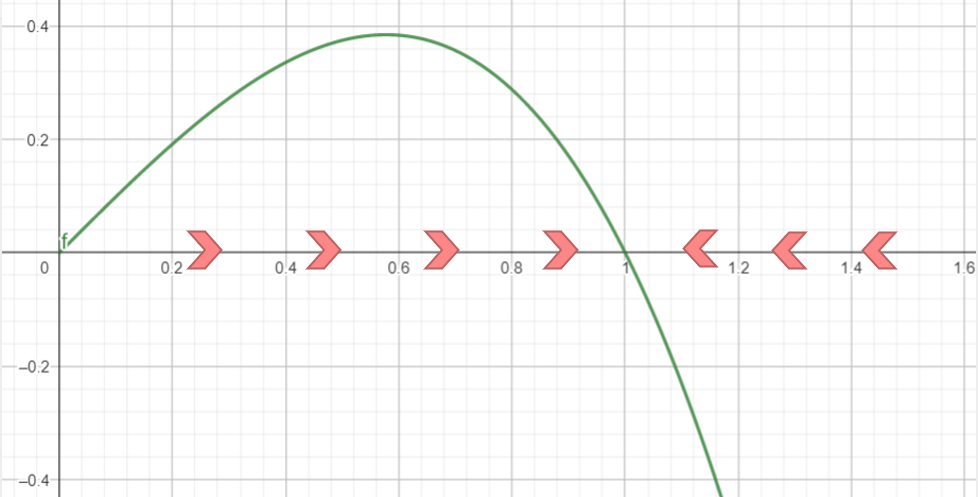
\includegraphics[width=14cm]{rej1.png}
	\caption{Plano fase de \eqref{eq: drsis1}.}
\end{figure}\\

Por otro lado para $\eqref{eq: dthetasis1}$ la solución es $\theta(t)=t+\theta_0$,
donde $\theta_0=\theta(0)$.\\

Las soluciones del sistema $\eqref{eq: sis1}$ convergen a puntos sobre la
circunferencia centrada en el origen de radio $1$ \cite{wiggins2003introduction}.\\

Resolvamos el problema de forma analítica.\\

La ecuación $\eqref{eq: drsis1}$ es separable
$$\int\frac{dr}{r(1-r^2)}=\int dt$$
integramos por fracciones parciales

$$\int\frac{dr}{r(1-r^2)}=\int\frac{dr}{r}-\int\frac{dr}{2(r+1)}-\int\frac{dr}{2(r-1)}$$
$$=\ln |r|-\frac{1}{2}\ln|r+1|-\frac{1}{2}\ln|r-1|+c_1$$

entonces
$$\ln |r|-\frac{1}{2}\ln|r+1|-\frac{1}{2}\ln|r-1|=t+c$$

desarrollamos logaritmos
$$\ln\left\lvert\frac{r^2}{r^2-1}\right\rvert=2t+c$$
$$\frac{r^2}{r^2-1}=ce^{2t}$$

$$r^2=\frac{e^{2t}}{c+e^{2t}}$$

Como $r\geq 0$
$$r=\frac{e^t}{\sqrt{c+e^{2t}}}$$
Aplicamos la condición inicial $r(0)=r_0$.\\
\\Las soluciones en coordenadas polares son:
\begin{equation}\label{eq: rsis1}
	r(t)=\frac{e^t}{\sqrt{\frac{1}{r_0^2}-1+e^{2t}}}
\end{equation}
\begin{equation}\label{eq: thetasis1}
	\theta(t)=t+\theta_0
\end{equation}

Dejaremos nuestra solución en coordenadas polares para realizar el siguiente
análisis del comportamiento asintótico.\\
\begin{enumerate}
	\item Si $r_0=1$ tenemos las ecuaciones
	      $$r(t)=1$$
	      $$\theta(t)=t+\theta_0$$
	\item Por otro lado, si $r_0>1$.
	      $$\lim_{t\to\infty}r(t)=\lim_{t\to\infty}\frac{e^t}{\sqrt{\frac{1}{r_0^2}-1+e^{2t}}}=1$$
	      $$\lim_{t\to-\infty}r(t)=\lim_{t\to-\infty}\frac{e^t}{\sqrt{\frac{1}{r_0^2}-1+e^{2t}}}=\infty$$
	\item Para $0<r_0<1$.
	      $$\lim_{t\to\infty}r(t)=\lim_{t\to\infty}\frac{e^t}{\sqrt{\frac{1}{r_0^2}-1+e^{2t}}}=1$$
	      $$\lim_{t\to-\infty}r(t)=\lim_{t\to-\infty}\frac{e^t}{\sqrt{\frac{1}{r_0^2}-1+e^{2t}}}=0$$
\end{enumerate}
Las trayectorias convergen a la circunferencia con centro en el origen
y de radio  $1$.\\

¿Qué significa que las trayectorias convergen a la circunferencia de centrada en el origen y de radio $1$?

\begin{definition} [Punto $\omega$ límite]
	Decimos que $\vec{z}\in\mathbb{R}^2$ es un punto $\omega$-límite
	de $\vec{x}_0\in\mathbb{R}^2$ si existe sucesión creciente de
	tiempos $\{t_n\}_{n\in\mathbb{N}}$
	con $t_n \to\infty$ cuando $n\to \infty$ tal que:
	$$\lim_{n\to\infty}\varphi^{t_n}(\vec{x}_0)=\vec{z}$$
\end{definition}

Pasemos las soluciones $\eqref{eq: rsis1}$ y $\eqref{eq: thetasis1}$ a coordenadas cartesianas, con $\eqref{eq: xpolar}$ y $\eqref{eq: ypolar}$ \cite{guckenheimer1983nonlinear}.
\begin{equation}\label{eq: xsis1}
	x(t)=\frac{e^t\cos(t+\theta_0)}{\sqrt{\frac{1}{r_0^2}-1+e^{2t}}}
\end{equation}
\begin{equation}\label{eq: ysis1}
	y(t)=\frac{e^t\sin(t+\theta_0)}{\sqrt{\frac{1}{r_0^2}-1+e^{2t}}}
\end{equation}
con $r_0=\sqrt{x_0^2+y_0^2}$ y $\theta_0=\arctan(\frac{y_0}{x_0})$. Definen el flujo $\varphi^t$ en $\mathbb{R}^2$ como
$$\varphi^t(x_0,y_0)=(x(t),y(t))$$

\begin{figure}[h]
	\centering
	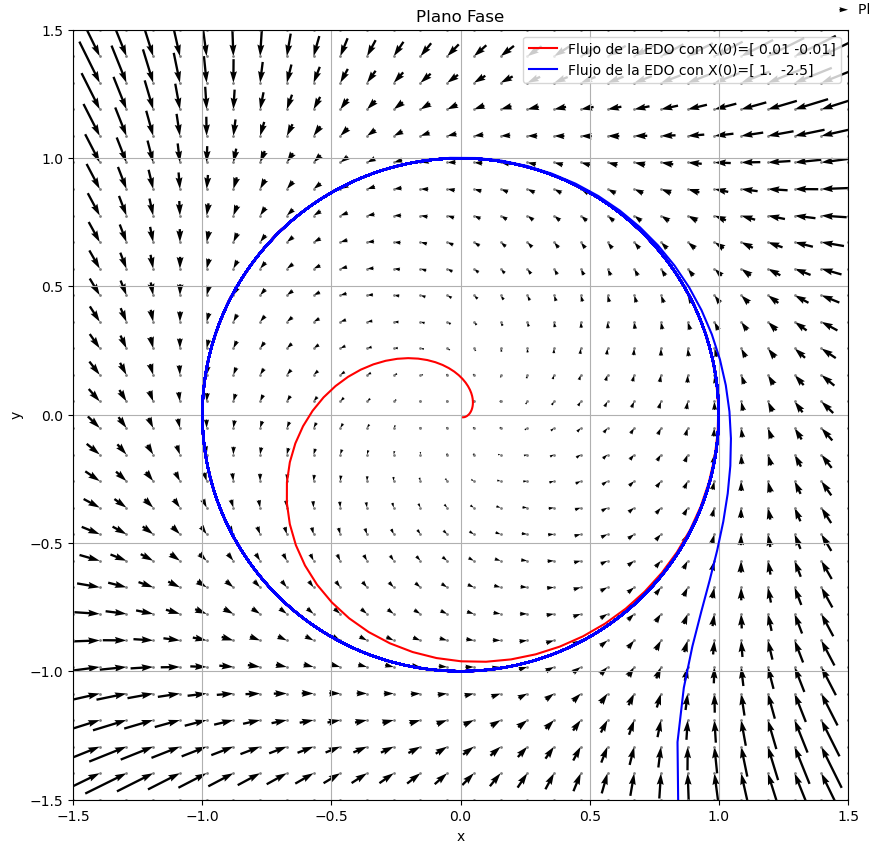
\includegraphics[width=13cm]{planofase1.png}
	\caption{Plano fase del sistema $\eqref{eq: sis1}$.}
\end{figure}

en el plano fase de $\eqref{eq: sis1}$ que pasa por el punto
$(x_0,y_0)$.\\

Tomemos un punto en la circunferencia centrada en el origen con radio $1$,
supongamos que
en coordenadas polares tiene un álgulo $0<\alpha_0<2\pi$, veamos que este punto es $\omega$ límite, para eso podemos definir
$\{t_n=2\pi n+\alpha_0-\theta_0\}_{n\in \mathbb{N}}$, entonces
$$\lim_{n\to\infty}x(t_n)=\cos(\alpha_0)$$
$$\lim_{n\to\infty}y(t_n)=\sin(\alpha_0)$$
en efecto el punto $(\cos(\alpha_0),\sin(\alpha_0))$ es un punto $\omega$ límite, esto
quiere decir que para cada punto de la circunferencia podemos encontrar
una sucesión de tiempos $\{t_n\}_{n\in \mathbb{N}}$ con $t_n\to\infty$ tal que la
trayectoria converge a ese punto de la circunferencia, es decir cualquier punto que se encuentra en la
circunferencia centrada en el origen y de radio $1$ es un punto $\omega$ límite de $(x_0,y_0)$,
entonces diremos que esta circunferencia es un conjunto $\omega$ límite de $(x_0,y_0)$, donde
el conjunto $\omega$ límite se define como

$$\omega(\vec{X}_0)=\{\vec{z}\in\mathbb{R}^2\mid\vec{z} \text{  es  } \omega\text{-límite de  } \vec{X}_0\}.$$

\begin{definition}[Punto $\alpha$ límite]
	Decimos que $\vec{z}\in\mathbb{R}^2$ es un punto $\alpha$-límite
	de $\vec{X}_0\in\mathbb{R}^2$ si existe sucesión decreciente de
	tiempos $\{t_n\}_{n\in\mathbb{N}}$
	con $t_n \to-\infty$ cuando $n\to \infty$ tal que:
	$$\lim_{n\to\infty}\varphi^{t_n}(\vec{X}_0)=\vec{z}$$
\end{definition}

Por otro lado si tomamos un punto $(x_0,y_0)$ que no está en la circunferencia, entonces si  $r_0<1$ entonces $x(t)\to 0$ y $y(t)\to 0$ cuando $t\to-\infty$, por lo tanto el punto $(x_0,y_0)$ es un punto $\alpha$ límite, es decir que existe una sucesión de tiempos $\{t_n\}_{n\in \mathbb{N}}$ con $t_n\to-\infty$ tal que la trayectoria converge a ese punto.\\

Notemos que analizamos los flujos cuando $t\to\infty$ y $t\to-\infty$, es decir que analizamos el comportamiento asintótico de las soluciones. Se define la trayectoria media positiva como
$$\varGamma_{x_0}^{+}=\{x=\varphi(t,x_0)\mid t\geq0\}$$
y la trayectoria media negativa como
$$\varGamma_{x_0}^{-}=\{x=\varphi(t,x_0)\mid t\leq0\}$$

\begin{figure}[h]\label{fig: plano_fase}
	\centering
	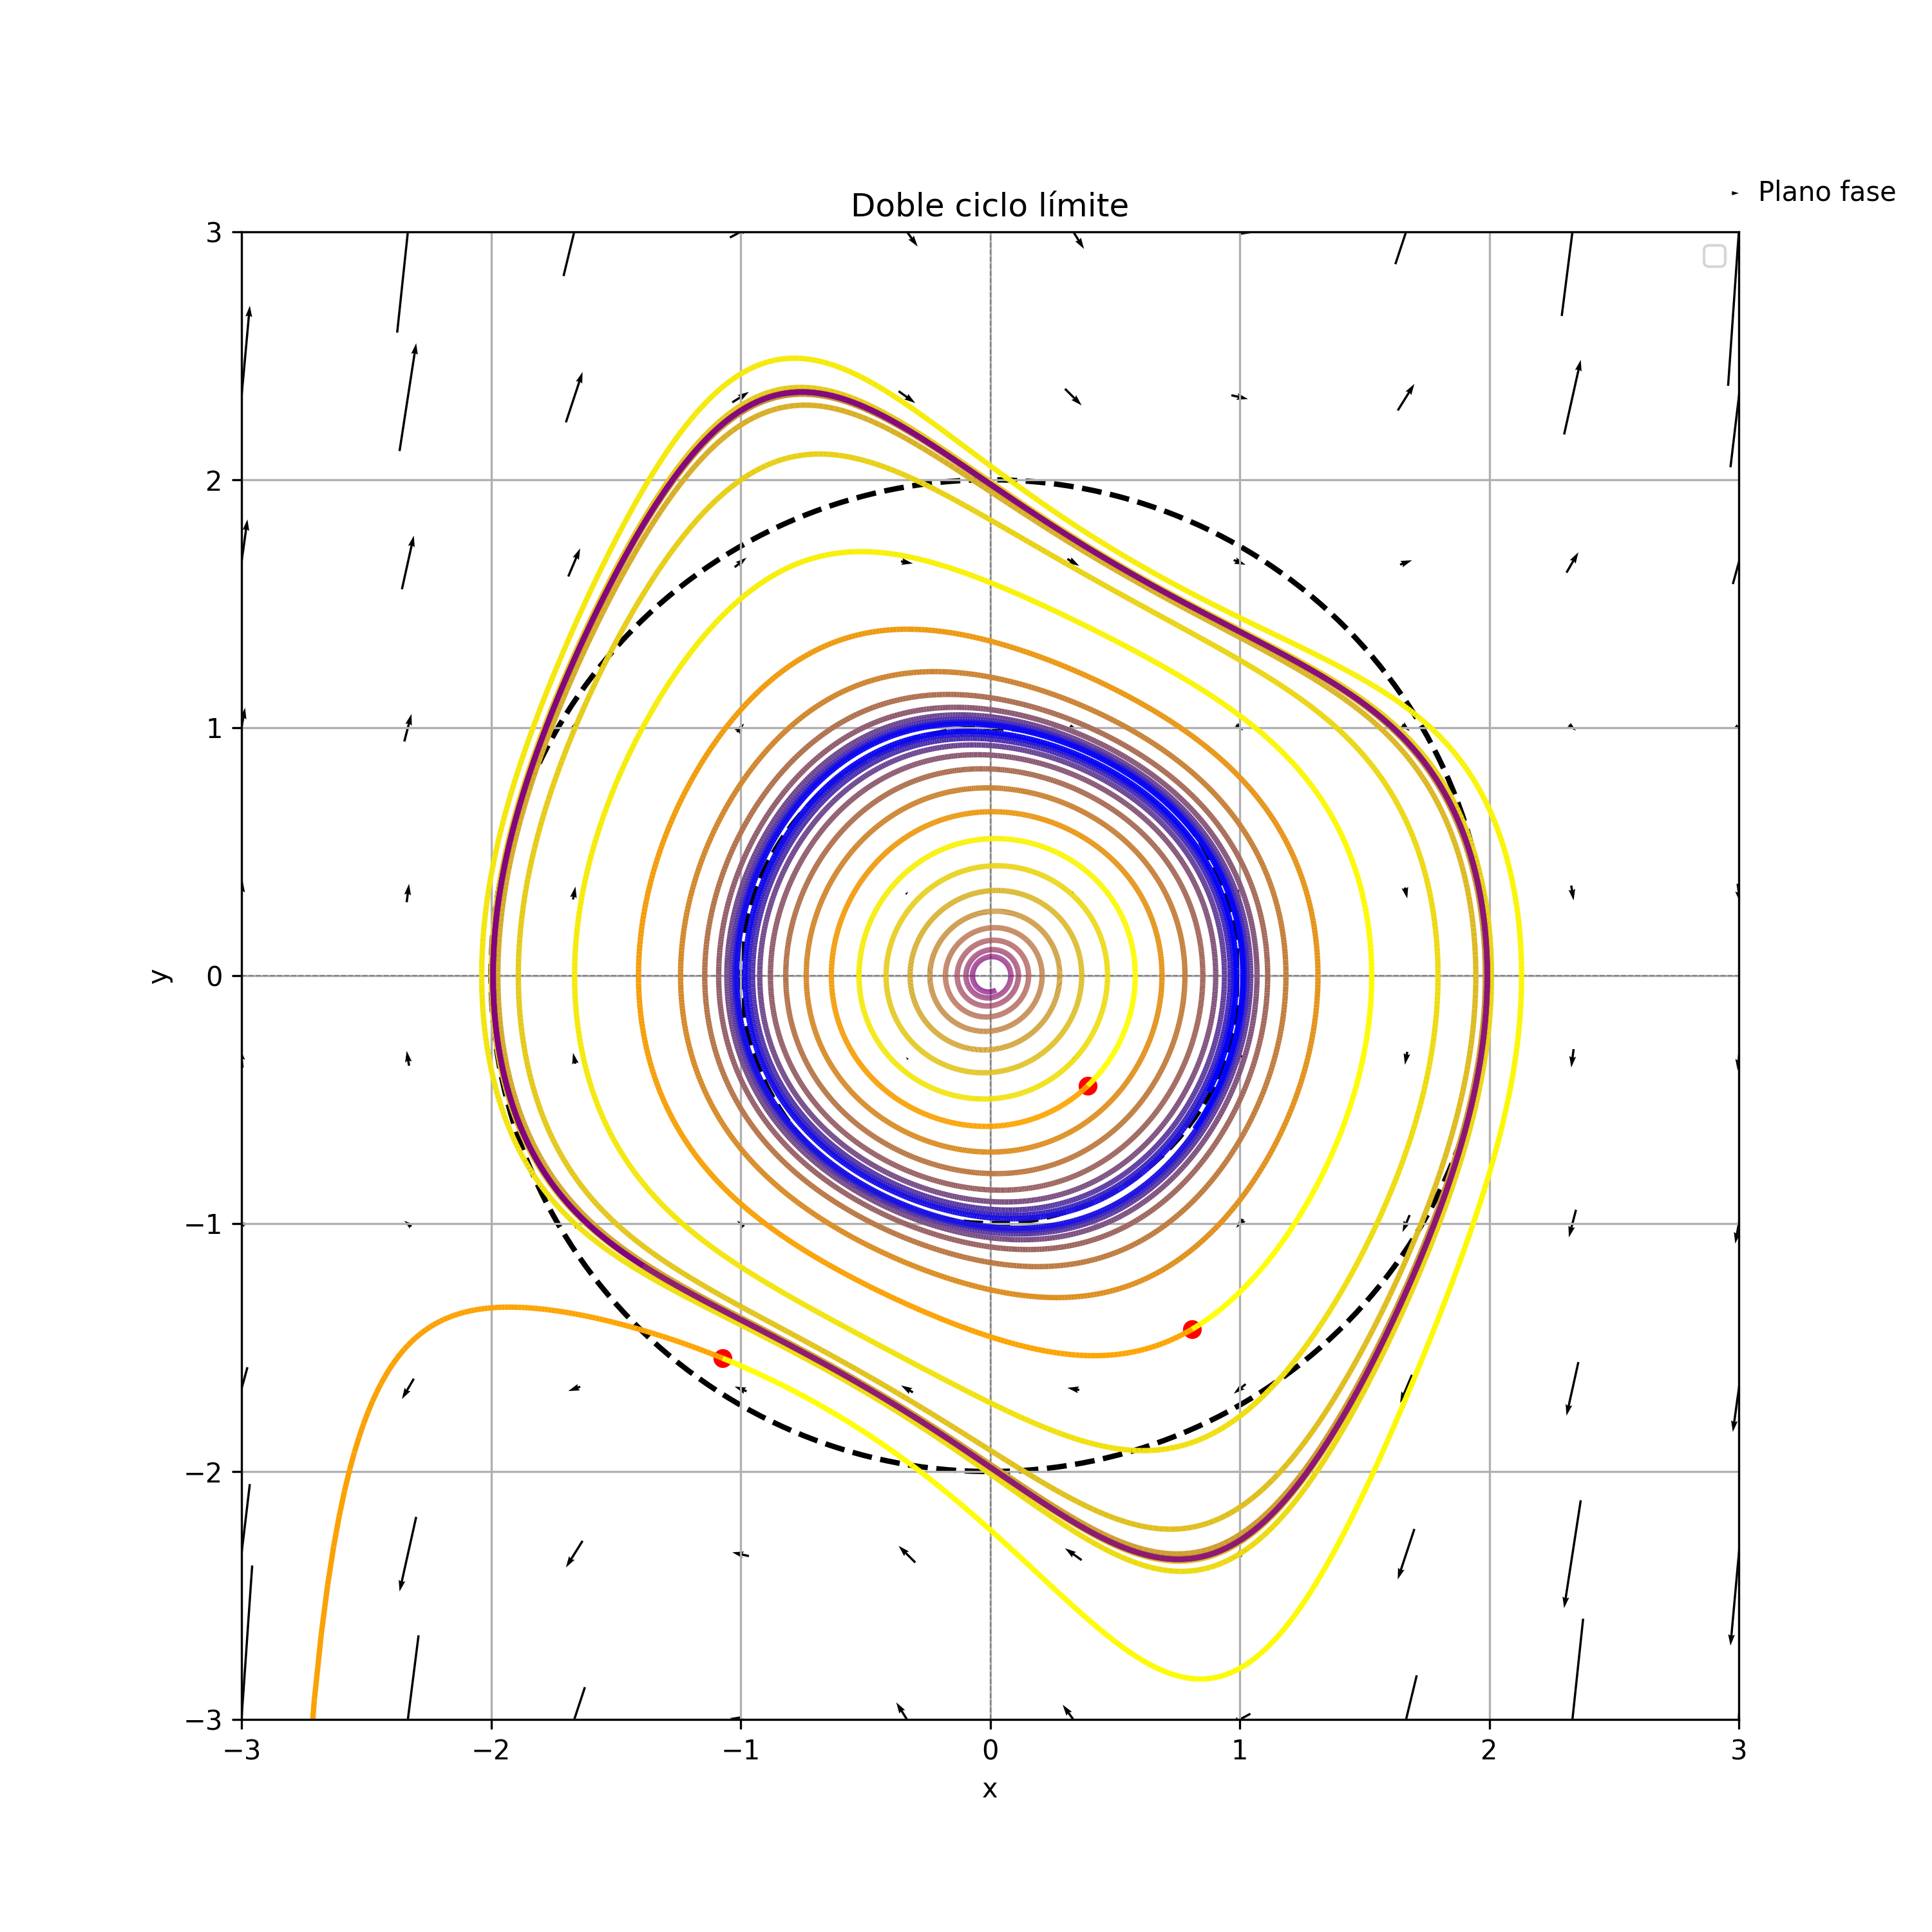
\includegraphics[width=12.5cm]{plano_fase.png}
	\caption{Plano fase del sistema $\eqref{eq: sis1}$.}
\end{figure}

En la figura \ref{fig: plano_fase} podemos observar que la trayectoria del flujo $\varphi^t$ que pasa por $x_0$ es la unión de la trayectoria media positiva (naranja) y la trayectoria media negativa (verde), es decir
$$\varGamma_{x_0}=\varGamma_{x_0}^{+}\cup\varGamma_{x_0}^{-}$$

\begin{definition}
	Decimos que un conjunto $U$ es positivamente invariante si dado $x_0\in U$ entonces  $\varGamma_{x_0}^{+}\subset U$
\end{definition}

\begin{definition}
	Decimos que un conjunto $U$ es negativamente invariante si dado $x_0\in U$ entonces  $\varGamma_{x_0}^{-}\subset U$
\end{definition}

Además, notemos que para $\{t_n=2\pi n+\alpha_0-\theta_0\}_{n\in \mathbb{N}}$,
la sucesión $\{(x(t_n),y(t_n))\}_{n\in\mathbb{N}}$ es una sucesión
de puntos convergente tal que sus puntos son colineales sobre la recta
$L=\{(x,y)\in\mathbb{R}^2\mid y=\tan(\alpha_0)x \}$. Las intersecciones de las trayectorias
son los valores de la sucesión colineal.\\

Modifiquemos el sistema $\eqref{eq: drsis1}$, a un sistema perturbado
con $0\leq\epsilon<1$.
\begin{equation}\label{eq: drmod}
	r'=r(1-r^2)+\epsilon r\cos(\theta)
\end{equation}
Veamos si existe $r_{max}$ tal que $r'<0$ y $r_{min}$ tal que $r'>0$ \cite{bender2013advanced}.\\

Reescribimos $\eqref{eq: drmod}$ como $r'=r(1-r^2+\epsilon \cos(\theta))$, como $r>0$,
entonces el signo de $r'$ depende de $1-r^2+\epsilon \cos(\theta)$.
Tenemos los siguientes casos:

\begin{enumerate}
	\item Si $1-r^2+\epsilon\cos(\theta)\leq 1-r^2+\epsilon<0$
	      entonces $\sqrt{1+\epsilon}<r_{max}$, por lo que para $r<r_{max}$ se tiene que $r'<0$.
	\item Por otro lado, si	$1-r^2+\epsilon\cos(\theta)>1-r^2-\epsilon>0$
	      entonces $\sqrt{1-\epsilon}>r_{min}$, por lo que para $r>r_{min}$ se tiene que $r'>0$.
\end{enumerate}

Las trayectorias que pasan por puntos en la circunferencia centrada
en el origen y con radio $r_{min}$
divergen del exterior de dicha circunferencia. Por otro lado,
las trayectorias que pasan por puntos en la circunferencia centrada
en el origen con radio $r_{max}$
convergen al interior del círculo.
A este segmento del plano lo llamamos región de atrapamiento \cite{hinch1991perturbation}.\\
\\Podemos intuir que debe existir
una curva cerrada en el interior, donde $r_{min}<r<r_{max}$, en la cual
las trayectorias convergen o alcanzan el equilibrio, de manera similar
a lo observado en el ejemplo
inicial, debido a su comportamiento. La idea de la existencia de una
curva cerrada de este tipo es lo que conocemos como ciclo límite.\\

\begin{figure}[h]
	\centering
	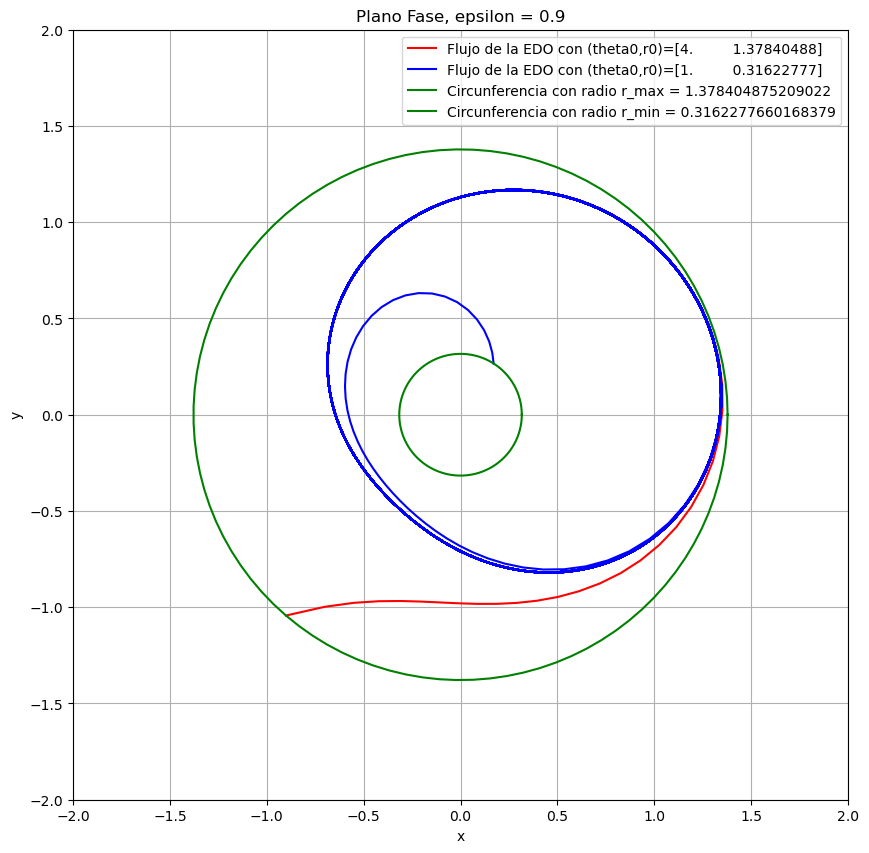
\includegraphics[width=13cm]{rminrmax.png}
	\caption{Plano fase del sistema con perturbación.}
\end{figure}

Notemos que esta sección del plano donde $r_{min}<r<r_{max}$ es positivamente invariante \cite{hirsch2012differential}.
\newpage

Veamos más propiedades de los puntos y el conjunto $\omega$ límite.

\begin{itemize}
	\item $\omega(x_0)=\omega(\varGamma_{x_0}^{+})$
	      y $\alpha(x_0)=\alpha(\varGamma_{x_0}^{-})$.\\
	\item Si $x_0$ es equilibrio de $x'=f(x)$ entonces:
	    $$\omega(x_0)=\alpha(x_0)=\{x_0\}$$
	\item Si $\varGamma_0$ es una órbita periódica para un sistema $x'=f(x)$, entonces
	      $$\omega(\varGamma_0)=\alpha(\varGamma_0)=\varGamma_0$$.
\end{itemize}

\begin{lemma}
	Sea $\vec{x}\in\mathbb{R}^n$ tal que $\Gamma_{x_0}^+$ está acotada.
	Entonces:
	\begin{enumerate}
		\item $\omega(x)\neq\emptyset$
		\item $\omega(x)$ es acotado.
		\item $\omega(x)$ es cerrado.
		\item $\omega(x)$ es conexo.
	\end{enumerate}
\end{lemma}

\begin{lemma}
	Sea $\vec{x}\in\mathbb{R}^n$ con $\Gamma_{x_0}^+$ acotada.
	Entonces
	$$\rho(\phi(t,x),\omega(\vec{x}))\to0$$
	cuando $t \to \infty$ \cite{hirsch2012differential}.
\end{lemma}

\begin{lemma}[Invarianza]
	Sea $\Gamma_{x_0}^+$ acotada. Entonces $\omega(x)$
	es invariante bajo el flujo
	$\varphi^t$, es decir, para cada $\vec{y}\in\omega(x)$ entonces
	$\varphi ^t(y)\in\omega(x)$ \cite{arnold1992ordinary}.
\end{lemma}

\begin{lemma}
	Si $\omega(x)\neq\emptyset$ y no contiene puntos de equilibrio. Entonces contiene una órbita periódica $\varGamma_0$ \cite{strogatz2018nonlinear}.
\end{lemma}

\begin{lemma}
	Si $\omega(x)$ contiene una órbita periódica $\varGamma_0$. Entonces $\omega(x)=\varGamma_0$ \cite{guckenheimer1983nonlinear}.
\end{lemma}

\section{Teorema de Poincaré-Bendixson}

\begin{theorem}[Poincaré-Bendixson]\label{TPB}
	Sea $x\in\mathbb{R}^2$ tal que $\varGamma_{x}^2\subseteq D\subseteq\mathbb{R}^2$ con $D\equiv$ Cerrado y acotado,
	y conteniendo un número finito de equilibrios de la EDO:
	\begin{equation}
		\begin{matrix}
			x' = f(x,y) \\
			y' = g(x,y)
		\end{matrix}
	\end{equation}
	entonces se cumple alguna de las siguientes:
	\begin{enumerate}
		\item $\omega(x)=\omega(\varGamma_{x}^+)$ está formado por un equilibrio.
		\item $\omega(x)$ es una órbita periódica.
		\item $\omega(x)$ está formada por equilibrios y órbitas que tienen a dichos equilibrios como puntos
		      $\alpha$ u $\omega$ límite.
	\end{enumerate}
\end{theorem}

El teorema de Poincaré-Bendixson es fundamental en la teoría de sistemas dinámicos planares \cite{poincare1881memoire,bendixson1901courbes}.

\begin{definition}[Ciclo límite.]
	Decimos que la órbita periódica $\varGamma_0=\omega(\vec{x})$
	del caso $2$ del teorema $\ref{TPB}$ se llama
	\textbf{ciclo límite} si hay un anillo abierto que lo
	contiene y no hay otra órbita periódica en él, es decir
	un ciclo límite es una órbita periódica aislada.
\end{definition}

\begin{definition}
	La órbita que conecta a un punto silla consigo mismo (la intersección de la variedad estable con la inestable), se le llama curva homoclínica \cite{kuznetsov2013elements}.
\end{definition}

\begin{definition}
	La órbita que conecta dos diferentes puntos de equilibrio se le llama curva heteroclínica \cite{kuznetsov2013elements}.
\end{definition}
\newpage

\section{Oscilador de Van der Pol}

La ecuación del oscilador de Van der Pol describe el comportamiento de ciertos sistemas oscilantes no lineales.
Su fundamento físico se basa en el concepto de amortiguamiento no lineal y autodemostración de oscilaciones \cite{vanderpol1926forced}.
\begin{equation}\label{eq: VP}
	x''+x+\epsilon x'(x^2-1)=0
\end{equation}
donde $\epsilon$ es un parámetro de amortiguamiento no lineal.\\
\\El término $-\epsilon(1 - x^2)x'$ representa la no linealidad del amortiguamiento en el sistema. La expresión
$(1 - x^2)$ describe cómo el amortiguamiento varía en función de la posición del oscilador. Cuando $x$ es
pequeño, este término es cercano a $1$ y el amortiguamiento es lineal. Sin embargo, a medida que $x$
aumenta, el término $(1 - x^2)$ se hace más negativo, generando un efecto de amortiguamiento no lineal que
disminuye la velocidad del oscilador \cite{strogatz2018nonlinear}.\\
\\Extendemos a un sistema de ecuaciones.
\begin{equation}\label{eq: VPsis}
	\begin{matrix}
		y'=-x-\epsilon y(x^2-1) \\
		x'=y
	\end{matrix}
\end{equation}

Los puntos de equilibrio del sistema se obtienen resolviendo \(x' = 0\) y \(y' = 0\):

\begin{equation}
    \begin{cases}
        y = 0, \\
        \epsilon (1 - x^2) y - x = 0.
    \end{cases}
\end{equation}

Sustituyendo \( y = 0 \) en la segunda ecuación, obtenemos:

\begin{equation}
    -x = 0 \implies x = 0.
\end{equation}

Por lo tanto, el único punto de equilibrio es el origen \((0, 0)\).

\subsubsection*{Matriz Jacobiana y Valores Propios}

Calculamos la matriz Jacobiana \( J \) del sistema \eqref{eq:van_der_pol_sistema}:

\begin{equation}
    J = 
    \begin{pmatrix}
        \dfrac{\partial x'}{\partial x} & \dfrac{\partial x'}{\partial y} \\
        \dfrac{\partial y'}{\partial x} & \dfrac{\partial y'}{\partial y}
    \end{pmatrix}
    =
    \begin{pmatrix}
        0 & 1 \\
        -1 - 2\epsilon x y & \epsilon (1 - x^2)
    \end{pmatrix}.
\end{equation}

Evaluando en el punto de equilibrio \((0, 0)\):

\begin{equation}
    J|_{(0,0)} = 
    \begin{pmatrix}
        0 & 1 \\
        -1 & \epsilon
    \end{pmatrix}.
\end{equation}

Obtenemos los valores propios \(\lambda\) resolviendo el determinante característico:

\begin{equation}
    \det(J - \lambda I) = 0,
\end{equation}

es decir,

\begin{equation}
    \left| \begin{array}{cc}
        -\lambda & 1 \\
        -1 & \epsilon - \lambda
    \end{array} \right| = 0.
\end{equation}

Calculamos el determinante:

\begin{equation}
    (-\lambda)(\epsilon - \lambda) - (-1)(1) = \lambda^2 - \epsilon \lambda + 1 = 0.
\end{equation}

Resolviendo la ecuación cuadrática:

\begin{equation}
    \lambda = \frac{\epsilon \pm \sqrt{\epsilon^2 - 4}}{2}.
\end{equation}

Para \(\epsilon > 0\), si \(\epsilon^2 - 4 > 0\) (es decir, \(\epsilon > 2\)), los valores propios son reales y positivos, lo que indica que el punto de equilibrio es un \textbf{nodo inestable}. Si \(0 < \epsilon < 2\), los valores propios son complejos con parte real positiva, lo que implica que el origen es un \textbf{foco inestable} \cite{guckenheimer1983nonlinear}.

\subsection*{Aplicación del Teorema de Poincaré-Bendixson}

Para demostrar la existencia de un ciclo límite, utilizamos el \textbf{teorema de Poincaré-Bendixson}, que establece que si un conjunto compacto, invariante y sin puntos de equilibrio en su interior existe para un sistema planar, entonces el sistema tiene una órbita periódica dentro de ese conjunto \cite{wiggins2003introduction}.

\subsubsection{Construcción de una Región Acotada Invariante}

Definimos una función de Lyapunov candidata:

\begin{equation}
    V(x, y) = \dfrac{1}{2} \left( x^2 + y^2 \right).
\end{equation}

Calculamos la derivada total de \( V \) respecto al tiempo:

\begin{equation}
    \dot{V} = x \dot{x} + y \dot{y} = x y + y \left( \mu (1 - x^2) y - x \right) = y^2 \left( \mu (1 - x^2) \right).
\end{equation}

Analizamos el signo de \( \dot{V} \):

\begin{itemize}
    \item Para \( |x| > 1 \), se tiene \( x^2 > 1 \), por lo que \( 1 - x^2 < 0 \) y entonces:

    \begin{equation}
        \dot{V} = y^2 \mu (1 - x^2) < 0.
    \end{equation}

    Esto indica que en la región donde \( |x| > 1 \), la energía total \( V \) decrece, y las trayectorias se dirigen hacia el interior de esta región.

    \item Para \( |x| < 1 \), se tiene \( 1 - x^2 > 0 \), y por lo tanto \( \dot{V} > 0 \), indicando que en esta región la energía total \( V \) aumenta, y las trayectorias se alejan del origen.
\end{itemize}

Concluimos que las trayectorias que empiezan fuera del círculo \( x^2 + y^2 = R^2 \) con \( R > 1 \) eventualmente entran en esta región y permanecen en un conjunto compacto y acotado \cite{hahn1967stability}.

Dado que:

\begin{enumerate}
    \item El sistema es plano y continuo.
    \item Existe una región compacta e invariante (por la función de Lyapunov) sin puntos de equilibrio distintos del origen.
    \item El origen es un punto de equilibrio inestable.
\end{enumerate}

Aplicando el teorema de Poincaré-Bendixson, concluimos que existe al menos una órbita periódica (ciclo límite) en la región acotada definida \cite{lasalle1961stability}.
\section{Ecuación de Rayleigh}
La ecuación de Rayleigh con amortiguamiento no lineal, se utiliza
para estudiar oscilaciones no lineales en sistemas mecánicos y se encuentra en
diversos campos como la mecánica estructural y la dinámica de sistemas físicos \cite{rayleigh1883theory}.

$$x''+\epsilon(x'^2-1)x'+x=0$$

El parámetro $\epsilon$ es un coeficiente que controla la influencia del término no lineal en el amortiguamiento.
El término $\epsilon(x'^2 - 1)x'$ es el término no lineal en el amortiguamiento. Mientras que en el amortiguamiento
lineal la fuerza de amortiguamiento es proporcional a la velocidad, en este caso el amortiguamiento depende de
la velocidad al cuadrado y se modifica por el término $(x'^2 - 1)$. Esto introduce un comportamiento no lineal en el
sistema y puede dar lugar a fenómenos como la autoexcitación y la respuesta no armónica \cite{strogatz2018nonlinear}.
Extendemos a un sistema de ecuaciones.

\begin{equation}\label{eq: Rayleigh}
	\begin{matrix}
		y'=-\epsilon(y^2-1)y-x \\ 
		x'=y
	\end{matrix}
\end{equation}

Los puntos de equilibrio se encuentran resolviendo \(\dot{x} = 0\) y \(\dot{y} = 0\):

\begin{equation}
    \begin{cases}
        y = 0, \\
        \epsilon \left(1 - y^2\right) y - x = 0.
    \end{cases}
\end{equation}

Sustituyendo \( y = 0 \) en la segunda ecuación, obtenemos:

\begin{equation}
    - x = 0 \implies x = 0.
\end{equation}

Por lo tanto, el único punto de equilibrio es el origen \((0, 0)\).

\subsubsection{Matriz Jacobiana y Valores Propios}

Calculamos la matriz Jacobiana \( J \) del sistema \eqref{eq: Rayleigh}:

\begin{equation}
    J =
    \begin{pmatrix}
        \dfrac{\partial \dot{x}}{\partial x} & \dfrac{\partial \dot{x}}{\partial y} \\
        \dfrac{\partial \dot{y}}{\partial x} & \dfrac{\partial \dot{y}}{\partial y}
    \end{pmatrix}
    =
    \begin{pmatrix}
        0 & 1 \\
        -1 & \epsilon \left(1 - 3 y^2\right)
    \end{pmatrix}.
\end{equation}

Evaluamos en el punto de equilibrio \((0, 0)\):

\begin{equation}
    J|_{(0,0)} =
    \begin{pmatrix}
        0 & 1 \\
        -1 & \epsilon
    \end{pmatrix}.
\end{equation}

Los valores propios \(\lambda\) se obtienen resolviendo:

\begin{equation}
    \det(J - \lambda I) = \left| \begin{array}{cc}
        -\lambda & 1 \\
        -1 & \epsilon - \lambda
    \end{array} \right| = 0.
\end{equation}

Calculamos el determinante:

\begin{equation}
    (-\lambda)(\epsilon - \lambda) - (-1)(1) = \lambda^2 - \epsilon \lambda + 1 = 0.
\end{equation}

Resolviendo la ecuación cuadrática:

\begin{equation}
    \lambda = \dfrac{\epsilon \pm \sqrt{\epsilon^2 - 4}}{2}.
\end{equation}

\begin{itemize}
    \item Si \(\epsilon^2 - 4 > 0\) (es decir, \(\epsilon > 2\)), los valores propios son reales y de signos opuestos si \(\epsilon > 0\), lo que indica un \textbf{silla de montar} en el origen.
    \item Si \(\epsilon^2 - 4 < 0\) (es decir, \(0 < \epsilon < 2\)), los valores propios son complejos conjugados con parte real positiva, ya que \(\epsilon > 0\). Esto implica que el origen es un \textbf{foco inestable}.
\end{itemize}

\subsection*{Aplicación del Teorema de Poincaré-Bendixson}

Para demostrar la existencia de un ciclo límite, aplicaremos el teorema de Poincaré-Bendixson, mostrando que las trayectorias están confinadas en una región acotada y que no hay otros puntos de equilibrio en esa región aparte del origen \cite{wiggins2003introduction}.

\subsubsection{Construcción de una Región Acotada Invariante}

Consideramos la siguiente función de Lyapunov candidata:

\begin{equation}
    V(x, y) = \dfrac{1}{2} y^2 + \dfrac{1}{2} x^2.
\end{equation}

Calculamos su derivada temporal:

\begin{align}
    \dot{V} &= y \dot{y} + x \dot{x} \\
    &= y \left[ \epsilon \left(1 - y^2\right) y - x \right] + x y \\
    &= y \left[ \epsilon \left(1 - y^2\right) y - x \right] + x y \\
    &= \epsilon y^2 \left(1 - y^2\right) - y x + x y \\
    &= \epsilon y^2 \left(1 - y^2\right).
\end{align}

Analizamos el signo de \(\dot{V}\):

\begin{itemize}
    \item Para \( |y| > 1 \), se tiene \( y^2 > 1 \), entonces \( 1 - y^2 < 0 \) y por lo tanto:

    \begin{equation}
        \dot{V} = \epsilon y^2 (1 - y^2) < 0.
    \end{equation}

    Esto indica que las trayectorias se dirigen hacia la región donde \( |y| \leq 1 \) \cite{hahn1967stability}.

    \item Para \( |y| < 1 \), se tiene \( 1 - y^2 > 0 \), y por lo tanto:

    \begin{equation}
        \dot{V} = \epsilon y^2 (1 - y^2) \geq 0.
    \end{equation}

    En esta región, la energía \( V \) no decrece, pero debido a la inestabilidad en el origen, las trayectorias tienden a alejarse del punto de equilibrio \cite{lasalle1961stability}.
\end{itemize}

Observamos que:

\begin{enumerate}
    \item Las trayectorias que empiezan fuera de la región \( |y| \leq 1 \) eventualmente entran en esta región y quedan confinadas en un conjunto compacto debido a la disminución de \( V \).

    \item No hay otros puntos de equilibrio distintos del origen en esta región.

    \item El origen es inestable (foco inestable o silla de montar dependiendo del valor de \(\epsilon\)).
\end{enumerate}

Por el \textbf{teorema de Poincaré-Bendixson}, existe al menos un ciclo límite en esta región acotada \cite{guckenheimer1983nonlinear}.
\section{Sistemas Liénard}

Los sistemas Liénard son ecuaciones diferenciales de la forma:
\begin{equation}\label{eq: lienard}
	x''+f(x)x'+g(x)=0
\end{equation}
Para extender esta ecuación diferencial a un sistema de ecuaciones diferenciales, primero definimos
$$F(x)=\int_0^x f(s)ds$$
entonces haciendo el cambio de variable $y=x'+F(x)$, obtenemos el sistema:
\begin{equation}\label{eq: lienardsystem}
	\begin{matrix}
		x'=y-F(x) \\
		y'=-g(x)
	\end{matrix}
\end{equation}
Vamos a enunciar el siguiente importante teorema \cite{lienard1928oscillations}.
\begin{theorem}[Liénard]
	Si $F(x)$ y $g(x)$ del sistema $\eqref{eq: lienardsystem}$ satisfacen las siguientes hipótesis:
	\begin{enumerate}
		\item $F,g\in C^1$.
		\item $F$ y $g$ son funciones impares.
		\item $xg(x)>0$ para todo $x\neq 0$.
		\item $F'(0)<0$
		\item $F$ tiene ceros sólo en $x=0$ o en $x=\pm a$.
		\item $F$ es monótona creciente en $(a,\infty)$ y $\lim_{x\to\infty}F(x)=\infty$
	\end{enumerate}
	entonces el sistema $\eqref{eq: lienardsystem}$ tiene un único ciclo límite y es estable \cite{perko2001differential}.
\end{theorem}
Veamos que el sistema de ecuaciones asociado al Oscilador de Van der Pol es un sistema Liénard.
$$x''+\epsilon(x^2-1)x'+x=0$$
Definimos
$$F(x)=\int_0^x \epsilon(s^2-1)ds$$
$$=\epsilon[\frac{1}{3}s^3-s]\big|_0^x=\epsilon[\frac{1}{3}x^3-x]$$
Tenemos $F(x)=\frac{\epsilon}{3}[x^3-3x]$ y $g(x)=x$.\\
\\Podemos extender el oscilador de Van der Pol al sistema de ecuaciones:
$$
	\begin{matrix}
		x'=y-\frac{\epsilon}{3}[x^3-3x] \\
		y'=-x
	\end{matrix}
$$
Veamos si $F$ y $g$ satisfacen las hipótesis del teorema de Liénard \cite{guckenheimer1983nonlinear}.
\begin{enumerate}
	\item En efecto $F,g\in C^1$.
	\item Notemos que las funciones son impares
	      $$F(-x)=\frac{\epsilon}{3}[(-x)^3-3(-x)]=\frac{\epsilon}{3}[-x^3+3x]=-\frac{\epsilon}{3}[x^3-3x]=-F(x)$$
	      $$g(-x)=-x=-g(x)$$.
	\item $xg(x)=x(x)=x^2>0$ para todo $x\neq 0$.
	\item $F'(0)=\epsilon(0^2-1)=-\epsilon<0$
	\item $F(x)=\frac{\epsilon}{3}[x^3-3x]=0$ entonces $F$ tiene raíces en $x=0$ y  $x=\pm \sqrt{3}$
	\item Si $y>x>\sqrt{3}$, entonces $y^3-3y>x^3-3x$, por lo que $F$ es monótona creciente. Además
	      por ser una función polinomial se tiene que
	      $$\lim_{x\to\infty}F(x)=\infty.$$
\end{enumerate}
Por lo tanto, por el teorema de Liénard el oscilador de Van der Pol tiene un único ciclo límite y es estable \cite{hale1980ordinary}.
Esto ya lo comprobamos anteriormente, pero este teorema nos garantiza que es el único ciclo límite \cite{khalil2002nonlinear}.
